\documentclass[12pt, a4paper, twoside]{report} % 12 pkt, A4, wydruk obustronny
\usepackage[utf8]{inputenc}
\usepackage{csquotes}
\usepackage[inner=2.5cm, outer=2.5cm, top=2.5cm, bottom=2.5cm]{geometry} % Marginesy po 2,5 cm
\usepackage{mathptmx} % Odpowiednik Times New Roman w LaTeX
\usepackage[T1]{fontenc}
\usepackage[polish]{babel}

\usepackage{setspace}
\onehalfspacing % Interlinia 1,5

\setlength{\parindent}{0.75cm} % Wcięcie akapitowe (np. 0,75 cm)
\usepackage[none]{hyphenat} % Wyłączenie dzielenia wyrazów
\sloppy % Pomaga w justowaniu przy wyłączonym dzieleniu wyrazów

\clubpenalty=10000 % Zabrania sierot (pierwszy wiersz akapitu na końcu strony)
\widowpenalty=10000 % Zabrania wdów (ostatni wiersz akapitu na nowej stronie)

\usepackage{titlesec}
% Rozdział: bold 14 pkt
\titleformat{\chapter}[hang]{\normalfont\fontsize{14}{16}\bfseries}{\thechapter.}{1em}{}
\titlespacing*{\chapter}{0pt}{0pt}{20pt} % Domyślnie LaTeX zaczyna od nowej strony

% Podrozdział: bold 12 pkt
\titleformat{\section}{\normalfont\fontsize{12}{14}\bfseries}{\thesection.}{1em}{}

% Paragraf: bold 10 pkt
\titleformat{\subsection}{\normalfont\fontsize{10}{12}\bfseries}{\thesubsection.}{1em}{}

\usepackage{caption}
\usepackage{float}
\usepackage{graphicx}

% Formatowanie podpisów (wielkość 11 pkt)
\captionsetup{font=small, labelsep=period} % small przy 12pt daje ok. 11pt

% Numeracja stron na środku w stopce (domyślne w klasie report w stylu plain)
\pagestyle{plain}

% Formatowanie podpisów (wielkość 11 pkt, tytuł bez kropki, odpowiednie pozycjonowanie)
\captionsetup[table]{font=small, labelsep=period, position=top} 
\captionsetup[figure]{font=small, labelsep=period, position=bottom}
\usepackage{longtable} % Umożliwia łamanie tabel między stronami i powtarzanie nagłówków
\usepackage[bottom]{footmisc} % Gwarantuje, że przypisy zawsze „przykleją” się do samego dołu strony
\usepackage[backend=biber, style=verbose-trad1]{biblatex} % Automatycznie obsłuży skróty typu "Ibidem"
\addbibresource{bibliografia.bib} % Ścieżka do Twojego pliku z literaturą

\begin{document}

\chapter{Zbiory danych}

\section{Charakterystyka zbioru MNIST}
Pierwszym obiektem, na którym przeprowadzono badania jest popularny w uczeniu maszynowych zbiór danych MNIST (ang. \textit{Modified National Institute of Standards and Technology}). Składający się łącznie około 70 000 obrazów (60 000 przykładów testowych oraz około 10 000 przykładów treningowych), przedstawia ręcznie pisane cyfry od 0 do 9. Każdy z obrazów domyślnie posiada rozmiar 28x28 pikseli, co w efekcie daje 784 piksele (cechy) dla każdego rozważanego obrazu. Cały zbiór danych reprezentowany jest w skali szarości, co oznacza, że każdy piksel przyjmuje wartość z zakresu od 0 do 255, gdzie 0 oznacza kolor czarny, natomiast 255 kolor biały. Przykładowe obrazy z tego zbioru danych przedstawiono na rysunku \ref{fig:1_mnist_samples}.

\begin{figure}[htbp]
    \centering
    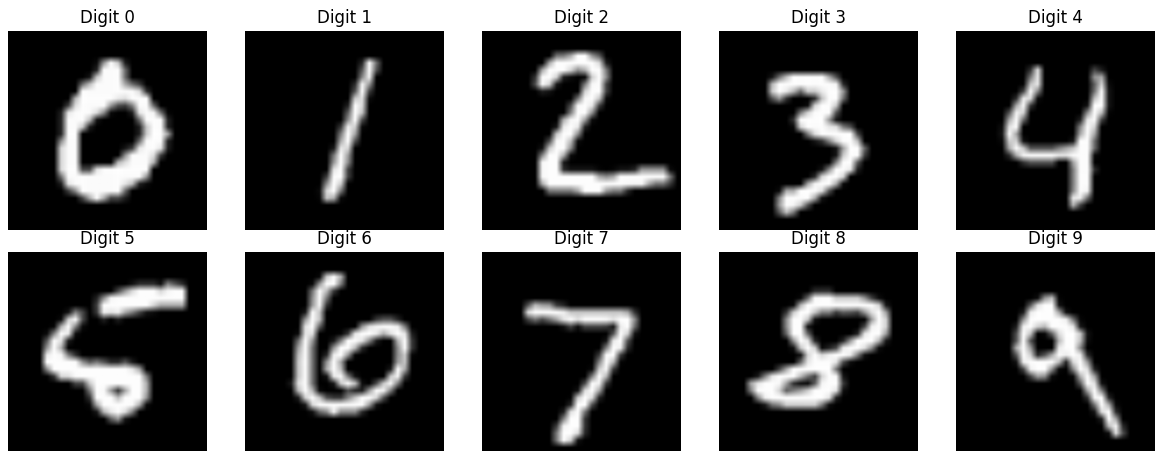
\includegraphics[width=0.7\textwidth]{imgs/1_mnist.png}
    \caption{Przykładowe obrazy z zbioru MNIST}
    \label{fig:1_mnist_samples}
\end{figure}

Cechą zbioru MNIST jest jego zbalansowany charakter, co oznacza, że każda z etykiet jest reprezentowana przez podobną ilość przykładów uczących w zbiorze. Zbalansowany zbiór danych jest kluczowy w zadaniach klasyfikacji, ponieważ pozwala na uniknięcie problemu tendencyjności modelu podczas późniejszej klasyfikacji nowych danych, których model wcześniej nie widział. Zdecydowano się na wykorzystanie opisywanego zbioru ze względu na jego popularność i prostotę. Skala szarości, która przekłada się na prostotę zbioru danych pozwala na wstępne zapoznanie się ze specyfiką wyników generowanych przez badane algorytmy wyjaśnialnej sztucznej inteligencji, co stanowi dobrą bazę do dalszych eksperymentów z bardziej złożonymi zbiorami danych.

\section{Charakterystyka zbioru CIFAR-10}

Kolejnym zbiorem danych, który wykorzystano w badaniach jest również popularny zbiór CIFAR-10 (ang. \textit{Canadian Institute for Advanced Research}). Zbiór ten charakteryzuje się podobną ilością przykładów, co omawiany wcześniej MNIST. Podobnie jak poprzednik, CIFAR-10 posiada 10 klas, jednak w w przeciwieństwie do MNIST, klasy te reprezentują różne obiekty, takie jak samochody, samoloty, ptaki etc. Od poprzednika różni się również rozmiarem obrazów. W tym przypadku mamy do czynienia z danymi o rozmiarze 32x32 pikseli, co daje 1024 cechy. Z racji, że CIFAR-10 jest zbiorem danych kolorowych, liczbę tę należy pomnożyć przez 3 (kanały RGB), co daje łącznie 3072 cechy dla każdego obrazu. Przykładowe obrazy z tego zbioru danych przedstawiono na rysunku \ref{fig:2_cifar_samples}.

\begin{figure}[htbp]
    \centering
    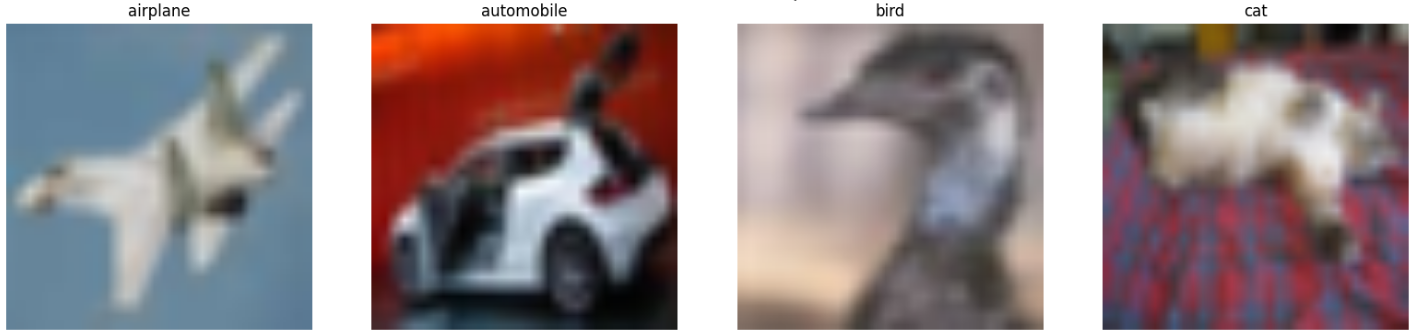
\includegraphics[width=0.7\textwidth]{imgs/2_cifar.png}
    \caption{Przykładowe obrazy z zbioru CIFAR-10}
    \label{fig:2_cifar_samples}
\end{figure}

Analogicznie jak w przypadku MNIST, CIFAR-10 jest zbiorem danych zbalansowanym, co oznacza, że każda z klas jest reprezentowana przez podobną ilość przykładów uczących. Wybór omawianego zbioru danych był podyktowany potrzebą zbadania algorytmów wyjaśnialnej sztucznej inteligencji w warunkach danych bardziej złożonych, które odzwierciedlają realistyczne scenariusze (różne gatunki zwierząt, obiekty, tło itp.). Ze względu na swoją różnorodność stanowi doskonały test dla badanych algorytmów, pozwalając na ocenę ich skuteczności w kontekście bardziej złożonych danych.

\chapter{Środowisko badawcze}

W niniejszym rozdziale przedstawiono wszystkie elementy środowiska badawczego, które zostały wykorzystane w przeprowadzonych eksperymentach. Opisano przygotowanie konfiguracji, danych, modeli klasyfikacyjnych, metod wyjaśniania decyzji modeli, metod generowania perturbacji oraz metryki oceny wyjaśnień. W całym eksperymencie zdecydowano się na podejście obiektowe i modułowe, co oznacza, że każdy z elementów środowiska badawczego został przygotowany w sposób niezależny, a następnie połączony w jedną całość. Takie podejście pozwoliło na elastyczność i możliwość łatwej modyfikacji poszczególnych elementów w przypadku potrzeby modyfikacji parametrów eksperymentu lub wprowadzenia nowych metod wyjaśniania decyzji modeli. W kolejnych sekcjach przedstawiono szczegółowe informacje dotyczące każdego z elementów środowiska badawczego, co pozwoli na pełne zrozumienie procesu przeprowadzonych eksperymentów oraz interpretację uzyskanych wyników.

\section{Przygotowanie konfiguracji, ścieżek oraz funkcji pomocniczych}
\label{sec:config_sciezki_utils}

Pracę nad środowiskiem badawczym rozpoczęto od zaimplementowania zestawu klas konfiguracyjnych oraz zestawu funkcji pomocniczych, których zadaniem było uporządkowanie parametrów eksperymentów i ograniczenie powtarzania tych samych fragmentów kodu w różnych częściach programu.

Do przechowywania parametrów wykorzystano klasy danych oznaczone dekoratorem \texttt{@dataclass}. Klasa \texttt{IGConfig} zawierała ustawienia metody Integrated Gradients, takie jak liczba kroków całkowania \texttt{n\_steps} oraz wartość bazowa \texttt{baseline\_value}. Wartość bazowa była wykorzystywana podczas tworzenia tensora odniesienia dla analizowanego obrazu. Klasa \texttt{OcclusionConfig} przechowywała parametry metody Occlusion. Zawierała osobne ustawienia dla zbiorów MNIST oraz CIFAR-10, obejmujące krok przesuwania okna \texttt{strides} oraz rozmiar okna okluzji \texttt{sliding\_window\_shapes}. Rozdzielenie tych parametrów pozwalało dostosować działanie metody do charakterystyki analizowanego zbioru danych. W klasie tej zdefiniowano również wartość bazową wykorzystywaną podczas zastępowania fragmentów obrazu.

Klasa \texttt{ExperimentConfig} grupowała parametry związane z przebiegiem eksperymentów. Obejmowała wartości odchylenia standardowego szumu Gaussa, wartości parametru \texttt{epsilon} dla ataku FGSM, procent pikseli uwzględnianych w metryce Top-K IoU, liczbę kroków w procedurze Deletion AUC oraz wartość bazową stosowaną podczas usuwania pikseli. Dzięki temu wszystkie najważniejsze parametry eksperymentalne były zebrane w jednym miejscu i mogły być łatwo modyfikowane bez ingerencji w kod poszczególnych klas. Klasa \texttt{TrainingConfig} zawierała podstawowe ustawienia procesu uczenia modelu, takie jak rozmiar batcha, liczba epok, współczynnik uczenia oraz udział zbioru walidacyjnego. Parametry te były wykorzystywane podczas przygotowywania danych oraz trenowania modeli klasyfikacyjnych. W projekcie zdefiniowano również klasę \texttt{Paths}, której zadaniem było przechowywanie ścieżek do najważniejszych katalogów projektu. Na podstawie lokalizacji pliku wyznaczano katalog główny projektu, a następnie katalog danych oraz katalog przeznaczony do zapisu modeli.

Dodatkowe funkcje pomocnicze umieszczono w pliku \texttt{utils.py}. Funkcja \texttt{get\_device()} automatycznie wybierała urządzenie obliczeniowe, zwracając GPU w przypadku dostępności technologii CUDA albo CPU w przeciwnym przypadku. Funkcja \texttt{tensor\_to\_img()} służyła do przekształcania tensora obrazu do postaci możliwej do wyświetlenia. W ramach tej operacji tensor był przenoszony na CPU, konwertowany do tablicy NumPy, a następnie przekształcany z zakresu wartości [-1,1] do zakresu [0,1]. Funkcja \texttt{plot\_image()} ujednolicała sposób wyświetlania obrazów i map atrybucji. Przyjmowała obiekt osi wykresu, obraz, tytuł oraz opcjonalne parametry mapy kolorów i zakresu wartości. Dzięki temu możliwe było stosowanie spójnego sposobu wizualizacji w różnych częściach eksperymentu. W pliku pomocniczym zdefiniowano także funkcję \texttt{initialize\_resnet18()}, która tworzyła model ResNet18. W zależności od przekazanego parametru model mógł zostać zainicjalizowany z wagami wstępnie wytrenowanymi lub bez nich. Ostatnia warstwa była zastępowana nową warstwą, której liczba wyjść odpowiadała liczbie klas analizowanego zbioru danych. Funkcja \texttt{load\_model\_weights()} umożliwiała wczytanie zapisanych wag modelu, przeniesienie modelu na odpowiednie urządzenie oraz przełączenie go w tryb ewaluacji.

\section{Przygotowanie danych oraz procesu trenowania}
\label{sec:dane_i_trening}

Następnie przystąpiono do przygotowania klasy \texttt{DataManager}, która służyła do ujednolicenia procesu przygotowania danych wykorzystywanych w badaniach. Jej głównym zadaniem było zapewnienie wspólnego interfejsu do obsługi zbioru MNIST oraz CIFAR-10, obejmującego pobieranie danych, ich wstępne przetwarzanie, wyodrębnienie ze zbioru treningowego zbioru walidacyjnego, pobranie zbioru testowego oraz obiektów Data Loader, które umożliwiały iterację po danych w trakcie trenowania modeli. Dzięki temu możliwe było łatwe zarządzanie danymi oraz zapewnienie spójności w procesie przygotowania danych dla eksperymentów.
W konstruktorze klasy określano ścieżkę do katalogu danych na podstawie klasy \texttt{Paths} oraz tworzono obiekt \texttt{TrainingConfig}, z którego pobierano parametry związane z treningiem, takie jak rozmiar batcha oraz udział zbioru walidacyjnego. Klasa przechowywała również mapowanie indeksów klas na ich nazwy. Dla zbioru MNIST indeksy odpowiadały cyfrom od 0 do 9, natomiast dla zbioru CIFAR-10 przypisano im nazwy klas, takie jak \texttt{airplane}, \texttt{automobile}, \texttt{bird} czy \texttt{cat}. Metoda \texttt{get\_class\_names()} umożliwiała pobranie tego mapowania dla wskazanego zbioru danych.

Istotnym elementem klasy \texttt{DataManager} jest metoda \texttt{get\_transform()}, która definiuje sposób przetwarzania obrazów w zależności od zbioru danych. Obrazy są przekształcane do rozmiaru 224x224 pikseli, następnie zamieniane na obiekty typu tensor. Ostatnim etapem przygotowywania danych dla modelu jest normalizacja. W badaniach została ona przeprowadzona zgodnie ze wzorem \ref{eq:x_norm}. 
\begin{equation} \label{eq:x_norm}
    x_{norm} = \frac{x - \mu}{\sigma}
\end{equation}
gdzie:
\begin{description}
    \item $x$ -- wartość wejściowa piksela,
    \item $\mu$ -- średnia wartość pikseli dla danego zbioru,
    \item $\sigma$ -- odchylenie standardowe wartości pikseli.
\end{description}
Wartości $\mu$ i $\sigma$ zostały przyjęte na poziomie 0.5. Podstawiając te wartości do wzoru \ref{eq:x_norm} otrzymujemy:
\begin{equation} \label{eq:x_norm_final}
    x_{norm} = \frac{x - 0.5}{0.5} = 2x - 1
\end{equation} 
Po transformacji obrazów do obiektu typu tensor wartości pikseli zawierają się w przedziale [0, 1]. Podstawiając te wartości do wzoru \ref{eq:x_norm_final} otrzymujemy, że po normalizacji wartości pikseli zawierają się w przedziale [-1, 1]. Taka normalizacja pozwala na wycentrowanie danych wejściowych wokół zera, co może prowadzić do stabilniejszego przebiegu procesu uczenia oraz efektywniejszej optymalizacji parametrów modelu. Należy również uwzględnić dodatkowy krok transformacyjny w przypadku zbioru MNIST. Ponieważ obrazy w tym zbiorze są jednokanałowe (skala szarości), konieczne było dodanie dodatkowego kroku transformacyjnego, który rozszerza pojedynczy kanał do trzech kanałów, ponieważ taki właśnie format wymagany jest przez architekturę sieci użytej w badaniach.

Metoda \texttt{get\_dataset()} pozwala na utworzenie odpowiedniego obiektu zbioru danych z biblioteki \texttt{PyTorch}, nakładając jednocześnie zdefiniowane wcześniej kroki transformacyjne. W celu wydzielenia zbioru walidacyjnego służącego do oceny modeli podczas procesu uczenia zaimplementowana została metoda \texttt{get\_train\_val\_datasets()}. Omawiana metoda pobiera pełny zbiór treningowy i wydobywa z niego zbiór walidacyjny o wielkości determinowanej przez parametr \texttt{val\_ratio}, który przyjęto na poziomie 0.1. Metoda \texttt{get\_test\_dataset()} stanowi wygodny sposób na pobranie zbioru testowego dla danego zbioru danych nakładając na niego odpowiednie transformacje. Ostatnią główną funkcjonalnością klasy \texttt{DataManager} jest metoda \texttt{get\_data\_loaders()}, która tworzy obiekty \texttt{DataLoader} dla zbioru treningowego, walidacyjnego oraz testowego. Obiekty te umożliwiają iterację po danych w trakcie trwania procesu uczenia modeli.

Po przygotowaniu klasy odpowiedzialnej za zarządzanie danymi przystąpiono do implementacji modułu \texttt{ModelTrainer}, którego zadaniem było uporządkowanie procesu treningu, walidacji oraz ewaluacji modeli klasyfikacyjnych wykorzystywanych w badaniach. Klasa ta pozwalała oddzielić logikę uczenia modelu od pozostałych elementów projektu.

Obiekt klasy \texttt{ModelTrainer} przyjmował model sieci neuronowej, urządzenie wykonujące obliczenia oraz nazwy klas występujących w analizowanym zbiorze danych. W konstruktorze określano również ścieżkę zapisu modelu na podstawie klasy \texttt{Paths} oraz tworzono obiekt \texttt{TrainingConfig}, z którego pobierano parametry konieczne do przeprowadzenia treningu. Funkcja straty została zdefiniowana jako \texttt{CrossEntropyLoss}, natomiast jako optymalizator wykorzystano algorytm \texttt{Adam}. Model był następnie przenoszony na wskazane urządzenie obliczeniowe. Klasa przechowywała również historię procesu uczenia w postaci słownika zawierającego wartości funkcji straty oraz dokładności dla zbioru treningowego i walidacyjnego. Dzięki temu możliwa była późniejsza analiza przebiegu uczenia modelu. 

Metoda \texttt{train\_one\_epoch()} realizowała pojedynczą epokę treningową. Dla kolejnych batchy wykonywana była propagacja w przód, obliczanie funkcji straty, propagacja wsteczna oraz aktualizacja wag modelu. Dla każdej epoki obliczana była średnia wartość funkcji straty oraz dokładność klasyfikacji na zbiorze treningowym. W metodzie \texttt{validate()} dokonywana była ocena modelu na zbiorze walidacyjnym w danej epoce. Wynikiem działania metody były średnia strata walidacyjna oraz dokładność klasyfikacji na zbiorze walidacyjnym. Metoda \texttt{fit()} pełniła rolę orkiestratora dwóch poprzednich metod, wywołując je w pętli po liczbie zadanych epok treningowych. Wyniki metod \texttt{train\_one\_epoch()} i \texttt{validate()} zapisywane były w historii treningu. Informacje w niej zawarte, czyli dokładność oraz wartości funkcji straty, były wykorzystywane do oceny jakości procesu uczenia. Po zakończeniu treningu model mógł zostać oceniony na zbiorze testowym za pomocą metody \texttt{evaluate()}, która generowała predykcje dla wszystkich przykładów testowych oraz raport klasyfikacyjny zawierający metryki dla poszczególnych klas. Ostatnią funkcjonalnością klasy \texttt{ModelTrainer} była metoda \texttt{save\_model()}, która umożliwiała zapis wag modelu do pliku, dając możliwość załadowania i wykorzystania modelu w późniejszych badaniach.

\section{Metody generowania perturbacji}
\label{sec:metody_generowania_perturbacji}

W celu generowania zakłóconych wersji obrazów wejściowych wykorzystywanych w eksperymentach nad stabilnością metod XAI zaimplementowano klasę \texttt{Perturbations}. Jej zadaniem było przygotowanie danych poddanych perturbacjom, które następnie wykorzystywano do porównania map atrybucji uzyskanych dla obrazów oryginalnych oraz zaburzonych.

Obiekt klasy \texttt{Perturbations} przyjmował model predykcyjny oraz urządzenie obliczeniowe. W konstruktorze określono również minimalną i maksymalną dopuszczalną wartość pikseli po perturbacji. Zgodnie z opisem procesu przygotowania danych w sekcji \ref{sec:dane_i_trening}, dane wejściowe zostały znormalizowane do zakresu [-1, 1], dlatego wartości graniczne ustawiono odpowiednio na -1 oraz 1. Po wygenerowaniu perturbacji wartości obrazu były ograniczane do tego przedziału, co zapewniało zgodność danych wejściowych z zakresem wykorzystywanym podczas trenowania modelu.

Pierwszą zaimplementowaną metodą perturbacji była metoda \texttt{gaussian()}, która dodawała do obrazu wejściowego szum Gaussa. W pierwszym kroku tworzono kopię tensora wejściowego i przenoszono ją na wybrane urządzenie obliczeniowe. Następnie generowano tensor losowego szumu o takim samym rozmiarze jak obraz wejściowy. Wygenerowany szum był skalowany przez parametr $\sigma$, a następnie dodawany do obrazu zgodnie ze wzorem \ref{eq:szum_gaussa}. Wynikowy tensor był ograniczany do zakresu [-1, 1] i zwracany jako zakłócona wersja obrazu wejściowego.

Drugą metodą perturbacji była metoda \texttt{fgsm()}, która generowała obraz zaburzony zgodnie z procedurą FGSM opisaną wzorem \ref{eq:fgsm}. Metoda przyjmowała tensor wejściowy, klasę docelową oraz wartość parametru $\epsilon$. Na początku tworzono kopię obrazu wejściowego, przenoszono ją na urządzenie obliczeniowe oraz włączano śledzenie gradientów względem wejścia. Następnie obraz przekazywano do modelu, a dla wskazanej klasy docelowej obliczano wartość funkcji straty. Po wyzerowaniu wcześniejszych gradientów wykonywano propagację wsteczną, dzięki czemu uzyskiwano gradient funkcji straty względem obrazu wejściowego. Na jego podstawie tworzono perturbację o skali określonej przez parametr $\epsilon$, którą dodawano do obrazu wejściowego. Po ponownym wyzerowaniu gradientów wynikowy obraz był ograniczany do zakresu [-1, 1] i zwracany jako przykład zaburzony. W obu metodach operacje wykonywane były na kopii tensora wejściowego, tak, aby oryginał został nienaruszony.

\section{Metody wyjaśniania decyzji modeli}
\label{sec:metody_wyjasniania_decyzji_modeli}

Kolejnym etapem przygotowywania środowiska badawczego było zaimplementowanie klas odpowiedzialnych za generowanie map atrybucji (wyjaśnień): \texttt{IGExplainer} oraz \texttt{OcclusionExplainer}. Obie klasy wykorzystywały implementacje metod dostępnych w bibliotece \texttt{Captum}, a ich zadaniem było ujednolicenie sposobu generowania wyjaśnień oraz przetwarzania otrzymanych atrybucji do formatu wykorzystywanego w dalszych eksperymentach. 

Klasa \texttt{IGExplainer} została zaimplementowana w celu generowania wyjaśnień metodą Integrated Gradients. Do konstruktora klasy przekazywano model predykcyjny oraz urządzenie obliczeniowe. Wewnątrz konstruktora tworzony był obiekt konfiguracyjny \texttt{IGConfig}, z którego pobierano parametry metody, takie jak liczba kroków \texttt{n\_steps}, która stanowiła przybliżenie całkowania ze wzoru \ref{eq:ig} oraz wartość bazowa \texttt{baseline\_value}. Dodatkowo inicjalizowano obiekt \texttt{IntegratedGradients} z biblioteki \texttt{Captum}, powiązany z analizowanym modelem.
Główną funkcjonalność klasy stanowiła metoda \texttt{explain()}, która przyjmowała tensor wejściowy oraz identyfikator klasy docelowej. Tensor wejściowy był przenoszony na wskazane urządzenie obliczeniowe, a następnie włączano dla niego śledzenie gradientów. Kolejnym krokiem było utworzenie tensora bazowego o takiej samej strukturze jak obraz wejściowy, wypełnionego wartością określoną w konfiguracji. Atrybucje wyznaczano za pomocą metody \texttt{attribute()}, do której przekazywano obraz wejściowy, tensor bazowy, klasę docelową oraz liczbę kroków określoną w \texttt{IGConfig}.

Klasa \texttt{OcclusionExplainer} pełniła analogiczną rolę dla metody Occlusion. Do jej konstruktora przekazywano model predykcyjny, urządzenie obliczeniowe oraz nazwę analizowanego zbioru danych. Wewnątrz klasy tworzony był obiekt \texttt{OcclusionConfig}, zawierający parametry metody osobno dla zbiorów MNIST oraz CIFAR-10. Inicjalizowano również obiekt \texttt{Occlusion} z biblioteki \texttt{Captum}. W metodzie \texttt{explain()} klasy \texttt{OcclusionExplainer} tensor wejściowy przenoszono na urządzenie obliczeniowe oraz tworzono tensor bazowy wypełniony wartością \texttt{baseline\_value}. Następnie, w zależności od wartości pola \texttt{dataset}, wybierano odpowiednie parametry \texttt{strides} oraz \texttt{sliding\_window\_shapes}. Atrybucje wyznaczano następnie za pomocą metody \texttt{attribute()}, przekazując do niej tensor wejściowy, parametry okna, tensor bazowy oraz klasę docelową.

Metoda ta agregowała atrybucje wyznaczone dla poszczególnych kanałów obrazu do jednej mapy atrybucji oraz przygotowywała trzy warianty reprezentacji wyniku: \texttt{raw}, \texttt{abs} i \texttt{deletion}. Pierwszy wariant zachowywał oryginalny znak atrybucji, drugi przedstawiał ogólną siłę wpływu niezależnie od znaku sumując wartości bezwzględne, natomiast trzeci pozostawiał jedynie dodatnie wartości atrybucji. Tak przygotowane mapy były następnie wykorzystywane w metrykach oceny stabilności wyjaśnień modeli.

\section{Metryki oceny wyjaśnień}
\label{sec:metryki_oceny_wyjaśnien}

W celu mierzalnej oceny stabilności oraz użyteczności map atrybucji zaimplementowano klasę \texttt{Metrics}. Klasa ta zawierała zestaw metod obliczających metryki wykorzystywane w dalszych eksperymentach. 

Pierwszą zaimplementowaną metryką było podobieństwo cosinusowe, realizowane przez metodę \texttt{cosine\_similarity()}. Metoda przyjmowała dwie mapy atrybucji, które w pierwszym kroku były przekształcane do postaci jednowymiarowych wektorów. Następnie obliczano stosunek ich iloczynu skalarnego do iloczynu długości obu wektorów zgodnie ze wzorem \ref{eq:cos_sim}. W celu zabezpieczenia obliczeń przed potencjalnym błędem dzielenia przez zero do mianownika dodawano niewielką stałą \texttt{1e-8}.

Drugą zaimplementowaną metryką była Top-K IoU, obliczana przez metodę \texttt{topk\_iou()}. Podobnie jak w przypadku podobieństwa cosinusowego, mapy atrybucji były najpierw przekształcane do postaci jednowymiarowych wektorów. Następnie na podstawie parametru \texttt{top\_k\_percent} wyznaczano liczbę pikseli należących do grupy najbardziej istotnych elementów. Dla każdej mapy wybierano indeksy pikseli o najwyższych wartościach atrybucji, a wartość metryki wyznaczano jako stosunek liczności części wspólnej tych zbiorów do liczności ich sumy.

Ostatnią zaimplementowaną metryką była Deletion AUC, której obliczanie realizowała metoda \texttt{deletion\_auc()}. Jej działanie rozpoczynało się od utworzenia kopii obrazu wejściowego oraz uporządkowania pikseli zgodnie z ich istotnością określoną przez przekazaną mapę atrybucji. Następnie, w kolejnych krokach, najbardziej istotne piksele były stopniowo zastępowane wartością bazową. Liczbę etapów tego procesu określał parametr \texttt{steps}, natomiast domyślną wartość bazową przyjęto na poziomie -1, zgodnie z zakresem wartości danych po normalizacji.
Po każdej modyfikacji obrazu wyznaczano prawdopodobieństwo przypisane przez model klasie docelowej i zapisywano je wraz z odpowiadającym mu udziałem usuniętych pikseli. Na podstawie otrzymanych wartości konstruowano krzywą opisującą zmianę pewności modelu wraz ze wzrostem liczby usuniętych pikseli, a następnie obliczano pole pod tą krzywą za pomocą funkcji \texttt{auc()} dostępnej w bibliotece \texttt{scikit-learn}.

\section{Orkiestracja eksperymentu}
\label{sec:orkiestracja_eksperymentu}

Głównym modułem odpowiedzialnym za przeprowadzanie eksperymentów była klasa \texttt{XAIExperiment}. Jej zadaniem była orkiestracja wcześniej przygotowanych elementów środowiska badawczego. Klasa ta umożliwiała przeprowadzenie kompletnej procedury porównywania wyjaśnień uzyskanych dla obrazów oryginalnych oraz ich zaburzonych wersji.

Do konstruktora klasy przekazywano model, urządzenie obliczeniowe, nazwy klas, zestaw poprawnie sklasyfikowanych przykładów oraz jeden z obiektów klas wyjaśniających opisanych w sekcji \ref{sec:metody_wyjasniania_decyzji_modeli}. Na podstawie przekazanych przykładów wyznaczano również listę analizowanych klas. Wewnątrz klasy tworzono obiekt \texttt{Perturbations}, odpowiedzialny za generowanie zaburzonych obrazów, obiekt \texttt{Metrics}, wykorzystywany do obliczania wartości metryk, oraz obiekt \texttt{ExperimentConfig}, zawierający parametry eksperymentów.

Metoda \texttt{iter\_clean\_examples()} umożliwiała iterację po wszystkich obrazach wykorzystywanych w eksperymencie. Dla każdej klasy zwracany był identyfikator klasy, numer przykładu oraz tensor obrazu przygotowany w formacie wymaganym przez model. Rozwiązanie to pozwalało wykonywać obliczenia nie tylko dla pojedynczego przykładu danej klasy, lecz także dla wielu przykładów, co umożliwiało późniejsze uśrednianie wyników.
Do generowania zaburzonych wersji obrazów wykorzystano metodę \texttt{get\_perturbed\_tensor()}. W zależności od wartości parametru \texttt{perturbation\_type} metoda wywoływała odpowiednią funkcję klasy \texttt{Perturbations}. Dla wartości \texttt{gaussian} generowany był obraz z dodanym szumem Gaussa, natomiast dla wartości \texttt{fgsm} tworzony był obraz zaburzony metodą FGSM.
Metoda \texttt{run\_similarity\_metrics()} odpowiadała za obliczanie metryk podobieństwa pomiędzy mapami atrybucji obrazów oryginalnych i zaburzonych. W pierwszym kroku tworzono pamięć podręczną map atrybucji dla obrazów oryginalnych, aby uniknąć ich wielokrotnego przeliczania dla każdej wartości perturbacji. Do obliczania podobieństwa wykorzystywano wariant mapy \texttt{abs}, czyli sumę wartości bezwzględnych atrybucji po kanałach obrazu. Wybór tego wariantu wynikał z celu analizowanych metryk. Podobieństwo cosinusowe oraz Top-K IoU miały oceniać przede wszystkim stabilność położenia obszarów istotnych dla modelu, a nie kierunek ich wpływu na predykcję. Z tego względu uwzględniano całkowitą siłę atrybucji niezależnie od jej znaku. 
Następnie dla kolejnych wartości parametru perturbacji generowano zaburzone obrazy, obliczano dla nich mapy atrybucji oraz porównywano je z wcześniej zapisanymi mapami obrazów oryginalnych. Wyniki zapisywano w postaci listy słowników zawierających typ perturbacji, wartość parametru, identyfikator klasy, nazwę klasy, numer przykładu oraz wartości obliczonych metryk. Ostatecznie wyniki zwracano jako obiekt \texttt{DataFrame} biblioteki \texttt{pandas}. Metoda \texttt{run\_deletion\_auc()} została przygotowana do oceny zmian wartości metryki Deletion AUC dla obrazów oryginalnych i zaburzonych. W tym przypadku wykorzystywano wariant mapy \texttt{deletion}, zawierający jedynie dodatnie wartości atrybucji. Taki wybór był związany z charakterem procedury Deletion AUC, w której kolejno zastępowano wartością bazową piksele uznane za najbardziej wspierające predykcję analizowanej klasy. Ujemne wartości atrybucji mogły oznaczać obszary działające przeciwnie względem danej klasy, dlatego nie były uwzględniane podczas wyboru pikseli usuwanych w tej metryce.
Podobnie jak w przypadku metryk podobieństwa, najpierw tworzono pamięć podręczną wyników dla obrazów oryginalnych. Dla każdego przykładu zapisywano predykcję modelu, pewność modelu względem klasy docelowej oraz wartość Deletion AUC obliczoną na podstawie mapy \texttt{deletion}. W dalszej części procedury, dla każdej wartości perturbacji, generowano obraz zaburzony i sprawdzano predykcję modelu oraz jego pewność względem klasy docelowej. Następnie wyznaczano mapę atrybucji dla obrazu zaburzonego i obliczano wartość Deletion AUC.

W klasie zaimplementowano również metody pomocnicze służące do agregacji wyników. Metoda \texttt{make\_pivot()} tworzyła tabelę przestawną, w której wartości wybranej metryki były uśredniane dla poszczególnych klas i poziomów perturbacji. Metoda \texttt{summarize\_similarity()} grupowała wyniki metryk podobieństwa względem wartości perturbacji i obliczała średnie oraz odchylenia standardowe dla podobieństwa cosinusowego i Top-K IoU. Analogicznie metoda \texttt{summarize\_deletion()} agregowała wyniki związane z Deletion AUC, pewnością modelu oraz liczbą zmian predykcji.

Zastosowanie klasy \texttt{XAIExperiment} pozwoliło uporządkować przebieg eksperymentów i zapewnić jednolity sposób obliczania wyników dla różnych metod wyjaśniania, typów perturbacji oraz analizowanych zbiorów danych.
\chapter{Analiza stabilności wyjaśnień dla zbioru MNIST}

\section{Integradient Gradients w obliczu szumu Gaussa}
\section{Integradient Gradients w obliczu ataków FGSM}
\section{Occlusion w obliczu szumu Gaussa}
\section{Occlusion w obliczu ataków FGSM}

\chapter{Analiza stabilności wyjaśnień dla zbioru CIFAR-10}


\section{Integradient Gradients w obliczu szumu Gaussa}
\section{Integradient Gradients w obliczu ataków FGSM}
\section{Occlusion w obliczu szumu Gaussa}
\section{Occlusion w obliczu ataków FGSM}

\chapter{Analiza porównawcza uzyskanych wyników}

\end{document}